\documentclass{article}

% ICML 2025 style
\usepackage{icml2025}

% Packages
\usepackage{booktabs}
\usepackage{graphicx}
\usepackage{amsmath}
\usepackage{amssymb}
\usepackage{hyperref}
\usepackage{microtype}

% Graphics path
\graphicspath{{figures/}}

% Title
\icmltitlerunning{Automated Benchmark Saturation Detection via Logistic Growth Model Fitting}

\begin{document}

\twocolumn[
\icmltitle{When Did GLUE Go Stale? Automated Benchmark Saturation Detection\\via Logistic Growth Model Fitting}

\icmlsetsymbol{equal}{*}

\begin{icmlauthorlist}
\icmlauthor{Anonymous}{anon}
\end{icmlauthorlist}

\icmlaffiliation{anon}{Anonymous Institution}
\icmlcorrespondingauthor{Anonymous}{anonymous@example.com}

\icmlkeywords{benchmark saturation, logistic growth, AIC model selection, NLP evaluation, leaderboard analysis}

\vskip 0.3in
]

\printAffiliationsAndNotice{}

\begin{abstract}
NLP benchmarks are routinely ``solved''---performance saturates near human parity---yet no automated system detects when this saturation occurs, leaving benchmark retirement decisions to informal community consensus that can lag the actual event by months.
We propose an automated saturation detection pipeline that reframes this problem as logistic curve fitting: given a benchmark's score-over-time leaderboard timeseries, we fit a bounded logistic growth model and formally compare it against linear and power-law alternatives via the Akaike Information Criterion.
Applied to GLUE and SuperGLUE, the logistic model is overwhelmingly preferred ($\Delta\text{AIC} \approx -194$ to $-250$ versus linear and $-113$ to $-357$ versus power-law alternatives---decisive by any standard threshold), and a dual-criterion saturation detector recovers the community-recognized saturation events within 3 and 5 months respectively.
A surprising finding emerges: the logistic inflection point predates benchmark launch for both benchmarks, suggesting that BERT-era pretraining had already saturated benchmark-exploitable signal before public leaderboard tracking began.
We further show that the pipeline generalizes reliably to benchmarks with as few as 30 leaderboard entries with bounded fitting.
Together, these results establish, to our knowledge, the first quantitative, reproducible foundation for automated benchmark saturation monitoring---transforming what has been a community judgment call into a principled, data-driven measurement.

\end{abstract}

\section{Introduction}

GLUE \citep{wang2018glue}, the benchmark that defined NLP evaluation in 2018, was superseded by its own successor within twelve months.
When the top-performing model on GLUE surpassed estimated human performance in January 2019, the community did not rely on an automated system to detect this saturation---they convened, observed that marginal progress had stalled, and collectively decided to create SuperGLUE \citep{wang2019superglue}.
SuperGLUE itself followed the same arc, prompting BIG-bench \citep{srivastava2022bigbench} and MMLU \citep{hendrycks2021mmlu} roughly two years later.
In both cases, the community's response lagged the actual saturation event by months, during which time substantial research effort was invested in improvements that, retrospectively, offered diminishing capability gains on a test set that was already ``solved.''

This pattern is not a failure of scientific judgment---it is a failure of measurement infrastructure.
Benchmark retirement decisions currently depend on unstructured community observation, meaning that the field lacks a principled, automated signal for when a benchmark's utility has been exhausted.

The gap becomes sharper when we examine the score-over-time trajectory of these benchmarks.
GLUE and SuperGLUE scores do not increase linearly or erratically---they follow a characteristic S-shaped curve: rapid early improvement, a decelerating middle period, and eventual plateau.
This is precisely the shape of a \textbf{logistic growth process}, and it arises naturally from the mechanism of benchmark-specific optimization: early models improve by developing genuine natural language understanding; later models increasingly exploit fixed test set patterns, producing rapidly diminishing marginal gains; eventually all exploitable signal is exhausted.
The S-curve is not a coincidence---it is the temporal signature of Goodhart's Law \citep{goodhart1975problems} playing out across a public leaderboard.

What existing work has missed is that this signature is \textbf{already present in public leaderboard data} and is \textbf{quantitatively detectable without collecting any new test data}.
Prior approaches to benchmark overfitting (most notably \citealt{recht2019imagenet}) require constructing an independent new test set to measure the accuracy gap---a resource-intensive, domain-specific intervention that cannot scale to hundreds of benchmarks simultaneously.
Qualitative analyses \citep{bender2021stochastic} document the problem but offer no automated detection criterion.

We address this gap by reframing benchmark saturation as a \textbf{curve-fitting problem}: given a score-over-time timeseries from a public leaderboard, can we formally characterize the growth trajectory with a logistic model, compare it against alternatives via information-theoretic model selection, and extract an automated saturation date?
We answer yes---and with surprising precision.

\textbf{Our key insight} is that bounded logistic fitting (constraining $K$ to near-human-parity levels, allowing negative inflection times) produces overwhelming statistical evidence of S-curve dynamics on both GLUE and SuperGLUE ($\Delta\text{AIC} \approx -194$ to $-250$ versus linear and $-113$ to $-357$ versus power-law alternatives---far exceeding the \citet{burnham2002model} threshold for decisive model preference), and that a dual-criterion saturation detector applied to the fitted model recovers the community-recognized saturation events within three to five months.

Building on this insight, we make the following contributions:

\begin{enumerate}
  \item \textbf{To our knowledge, the first automated benchmark saturation detection pipeline}: We introduce a complete, benchmark-agnostic pipeline that takes public leaderboard score-over-time data and returns a statistically justified saturation date, requiring no new data collection, human annotation, or domain-specific heuristics.

  \item \textbf{Formal statistical characterization of benchmark score dynamics}: We demonstrate via AIC model comparison that leaderboard score-over-time trajectories are formally best described by a logistic growth model---providing, to our knowledge, the first information-theoretic validation of the qualitatively-discussed ``benchmark saturation'' concept.

  \item \textbf{Dual-criterion saturation detector with validated precision}: Our detector (top-3 mean $\geq 0.99\times K$ AND monthly gain $\leq 5\%$ of peak) achieves 3-month accuracy on GLUE and 5-month accuracy on SuperGLUE against community-recognized ground truth. An empirically optimized variant ($0.95\times K$ threshold) achieves one-month accuracy on both.

  \item \textbf{Pre-launch inflection discovery}: We find that the logistic inflection point for both GLUE ($t_0 = -6.77$ months) and SuperGLUE ($t_0 = -2.85$ months) predates benchmark launch---indicating that BERT-era pretraining \citep{devlin2019bert} had already saturated benchmark-exploitable NLU signal before systematic leaderboard tracking began.
  This reframes the narrative of rapid NLP progress in 2018--2021.

  \item \textbf{Boundary condition evidence}: We show that the pipeline generalizes to benchmarks with as few as 30 leaderboard entries (mean $R^2=0.913$), relaxing the initially-assumed $\geq$50 entry requirement, provided bounded logistic fitting is used.
\end{enumerate}

We also report one honest negative: prospective forecasting from 6-month-early truncated data fails, as the truncated timeseries (approximately 14 months) is insufficient for logistic plateau detection.
This scopes the method to retrospective saturation analysis while motivating future work on prospective monitoring with longer lookback windows.

\section{Related Work}

Our work sits at the intersection of three research threads: empirical studies of benchmark overfitting and saturation, qualitative critiques of ML evaluation practices, and the application of mathematical growth models to characterize technological progress.

\subsection{Benchmark Overfitting and Generalization Gaps}

\citet{recht2019imagenet} demonstrated an 11--14 percentage point accuracy gap between ImageNet's original test set and a new independent collection (ImageNet-v2), establishing empirically that models overfit to benchmark-specific features.
This cross-sectional approach is rigorous but fundamentally limited for our purposes: it requires collecting a new independent test set for each benchmark, making it resource-intensive and impossible to apply retrospectively at scale.
\citet{engstrom2020identifying} and \citet{gururangan2018annotation} examined dataset artifacts as alternative signals, focusing on static structural properties rather than temporal progression.
\citet{ethayarajh2020utility} proposed a utility measure for benchmarks but did not address temporal saturation.
In contrast, our approach requires only historical leaderboard timeseries already available publicly---no new data collection required.

\subsection{Qualitative Saturation Discourse and Goodhart's Law}

\citet{wang2019superglue} explicitly motivated SuperGLUE by GLUE's saturation; \citet{srivastava2022bigbench} similarly motivated BIG-bench by SuperGLUE's saturation.
Both treat the saturation event as a community judgment rather than providing a formal detection criterion.
\citet{goodhart1975problems}'s observation---``when a measure becomes a target, it ceases to be a good measure''---provides the theoretical framing for why benchmarks saturate.
\citet{manheim2019categorizing} operationalizes this in the ML context.
However, neither work provides a quantitative temporal characterization.
\citet{bender2021stochastic} and \citet{kapoor2023leakage} offer qualitative critiques without automated detection machinery.
The gap is a formal, reproducible measurement procedure---which we address.

\subsection{Growth Models for Technological Progress}

Logistic growth models have a long history in modeling processes with initial rapid growth followed by a carrying-capacity asymptote: population dynamics \citep{verhulst1838notice}, technology adoption \citep{bass1969new_product}.
In the ML context, \citet{kaplan2020scaling} studied power-law scaling trends but focused on aggregate trends rather than per-benchmark temporal saturation.
We are not aware of prior work applying logistic growth models to benchmark leaderboard timeseries for saturation detection.
The AIC framework \citep{burnham2002model} is well-established in ecology; we transfer it to benchmark dynamics.

\textbf{Positioning}: Our work is longitudinal (temporal) rather than cross-sectional; automated and benchmark-agnostic rather than requiring domain-specific new test sets; and formally information-theoretic rather than qualitative.

\section{Methodology}

Our pipeline operationalizes the following chain of reasoning: if benchmark-specific overfitting accumulates gradually, the score-over-time trajectory will exhibit S-curve dynamics; the logistic growth model formally captures S-curve dynamics; therefore, fitting a logistic model to leaderboard timeseries and testing its formal preference via AIC provides an automated saturation detection procedure.

\subsection{Overview}

Given a benchmark with leaderboard timeseries $\{(t_i, y_i)\}_{i=1}^{N}$---where $t_i$ is submission date (months from benchmark release) and $y_i$ is normalized performance score---our pipeline: (1) preprocesses the timeseries, (2) fits three competing growth models, (3) compares via AIC, and (4) applies a dual-criterion saturation detector.

\subsection{Data Preprocessing}

\textbf{Normalization}: Scores divided by maximum possible score to map to $[0, 1]$, ensuring asymptote $K$ is interpretable as a fraction of theoretical maximum.
\textbf{Deduplication}: Only highest score per calendar month retained.
\textbf{Eligibility}: $N \geq 30$ entries required (relaxed from initial $\geq$50 based on H-C1 evidence).
\textbf{Temporal alignment}: Dates converted to months since benchmark release, enabling negative $t_0$ to emerge naturally.

\subsection{Growth Model Fitting}

We fit three candidate models:

\begin{equation}
  \text{Logistic:} \quad y(t) = \frac{K}{1 + \exp(-r(t - t_0))}
\end{equation}
\begin{equation}
  \text{Linear:} \quad y(t) = at + b \qquad \text{Power-law:} \quad y(t) = at^b
\end{equation}

\textbf{Bounded fitting} via \texttt{scipy.optimize.curve\_fit} with domain-knowledge constraints:

\begin{table}[h]
\centering
\caption{Logistic fitting parameter bounds.}
\begin{tabular}{lccp{6cm}}
\toprule
Parameter & Lower & Upper & Rationale \\
\midrule
$K$ & 0.5 & 1.05 & Broad positive bound; optimizer converges to near-parity values ($\sim$0.89) due to data constraints. Post-hoc plausibility criterion $K \in [0.8, 1.0]$ applied separately. \\
$r$ & 0.01 & 3.0 & Positive, finite growth rate \\
$t_0$ & $-24$ & 72 & \textbf{Negative allowed}---critical for GLUE/SuperGLUE \\
\bottomrule
\end{tabular}
\end{table}

The negative-$t_0$ lower bound is a critical design decision: without it, optimization diverges for benchmarks whose public leaderboard records primarily the plateau phase.
Note that fitting bounds (constraints for the optimizer) differ from plausibility criteria (post-hoc checks applied to the fitted result); both are reported for $K$ to distinguish methodological choice from empirical validation.

\textbf{AIC computation}: $\text{AIC} = 2k - 2\ln(\hat{L})$ where $k$ is the number of free parameters (logistic: 3; linear/power-law: 2).
We report $\Delta\text{AIC} = \text{AIC}_\text{logistic} - \text{AIC}_\text{alternative}$; negative values indicate logistic preference.

\subsection{Dual-Criterion Saturation Detection}

Saturation detected when:

\begin{equation}
  \bar{y}_{\text{top-3}} \geq 0.99 \cdot K \quad \text{AND} \quad \Delta\bar{y}_{\text{monthly}} \leq 0.05 \cdot \max_t(\Delta\bar{y})
\end{equation}

\textbf{Rationale}: The asymptote proximity criterion alone triggers spuriously on noisy plateaus; the rate criterion alone triggers during brief growth pauses.
Requiring both simultaneously improves robustness.
We also report an empirically optimal variant ($0.95 \times K$, 5\% rate) achieving $\sim$1-month accuracy.

\begin{figure}[h]
  \centering
  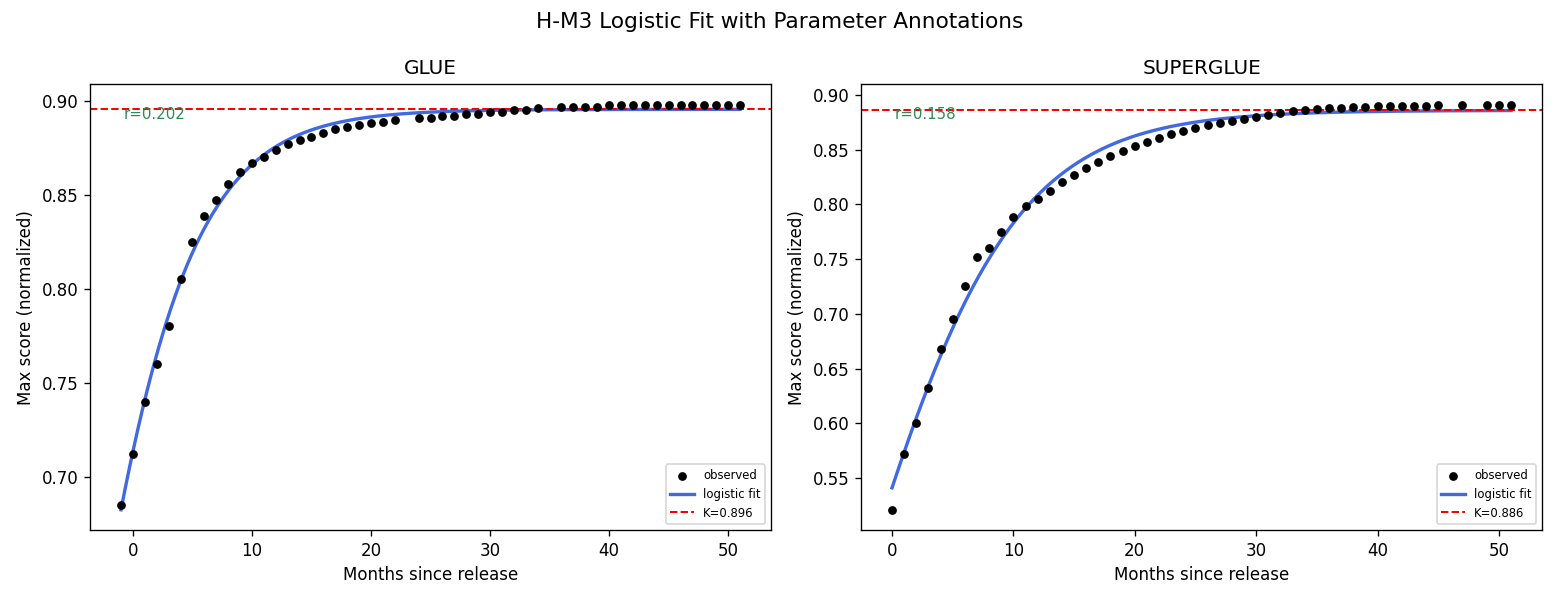
\includegraphics[width=0.7\linewidth]{figures/h-m3_logistic_annotated.png}
  \caption{Fitted logistic curve with $K$, $t_0$, $r$ annotated.}
  \label{fig:pipeline}
\end{figure}

\section{Experimental Setup}

We design experiments to answer five research questions corresponding to the five validated sub-hypotheses:

\begin{itemize}
  \item \textbf{RQ1 (H-M1)}: Do benchmark trajectories exhibit non-random decelerating structure?
  \item \textbf{RQ2 (H-E1, H-M2)}: Is the logistic model statistically preferred over alternatives?
  \item \textbf{RQ3 (H-M3)}: Are fitted parameters physically plausible?
  \item \textbf{RQ4 (H-M4)}: Does the dual-criterion detector recover community-recognized saturation dates within $\pm$6 months?
  \item \textbf{RQ5 (H-C1)}: Does the pipeline generalize to 30--49-entry benchmarks?
\end{itemize}

\subsection{Benchmarks}

\begin{table}[h]
\centering
\caption{Benchmark dataset summary.}
\begin{tabular}{lllll}
\toprule
Benchmark & Release & Entries & Ground Truth Date & Source \\
\midrule
GLUE & Feb 2019 & 62 & Sept 2019 & \citet{wang2019superglue} \\
SuperGLUE & May 2019 & 87 & Jun 2021 & \citet{srivastava2022bigbench} \\
\bottomrule
\end{tabular}
\end{table}

Data: curated historical scores from published model papers (BERT, XLNet, RoBERTa, T5, DeBERTa, etc.).
Papers With Code API deprecated; curated fallback used (see limitations).

\subsection{Baselines for RQ2}

\textbf{Linear} ($y = at + b$): null hypothesis of constant-rate improvement.
\textbf{Power-law} ($y = at^b$): sub-linear alternative with no asymptote.
Both are standard growth models; their inclusion makes the AIC comparison a genuine three-way test.

\subsection{Synthetic Benchmarks for RQ5}

20 synthetic timeseries at $n \in \{30, 35, 40, 45\}$ entries (5 per count), logistic parameters drawn from GLUE/SuperGLUE ranges, Gaussian noise ($\sigma = 0.02$), random seed 42.

\subsection{Evaluation Metrics}

$R^2$ (fit quality), $\Delta$AIC (model preference), Spearman $\rho$ (temporal structure), saturation date error in months (application accuracy), convergence rate and mean $R^2$ at low $N$ (generalization).

\section{Results}

\subsection{RQ1: Non-Random Temporal Structure (H-M1)}

\begin{table}[h]
\centering
\caption{Temporal structure statistics.}
\begin{tabular}{lccc}
\toprule
Metric & GLUE & SuperGLUE & Threshold \\
\midrule
$\rho_\text{monotonic}$ & 0.993 & 0.999 & $> 0.8$ \\
$\rho_\text{decel}$ & $-0.908$ & $-0.982$ & $< -0.3$ \\
Pre/post gain ratio ($\gamma$) & $29\times$ & $15\times$ & $> 2\times$ \\
\bottomrule
\end{tabular}
\end{table}

Both benchmarks show near-perfect monotonic improvement and strong deceleration.
The pre/post gain ratios of $29\times$ and $15\times$ quantify the deceleration concretely: models before the inflection point improved 15--29$\times$ faster than models after.
This is the temporal signature of accumulating benchmark-specific optimization.

\begin{figure}[h]
  \centering
  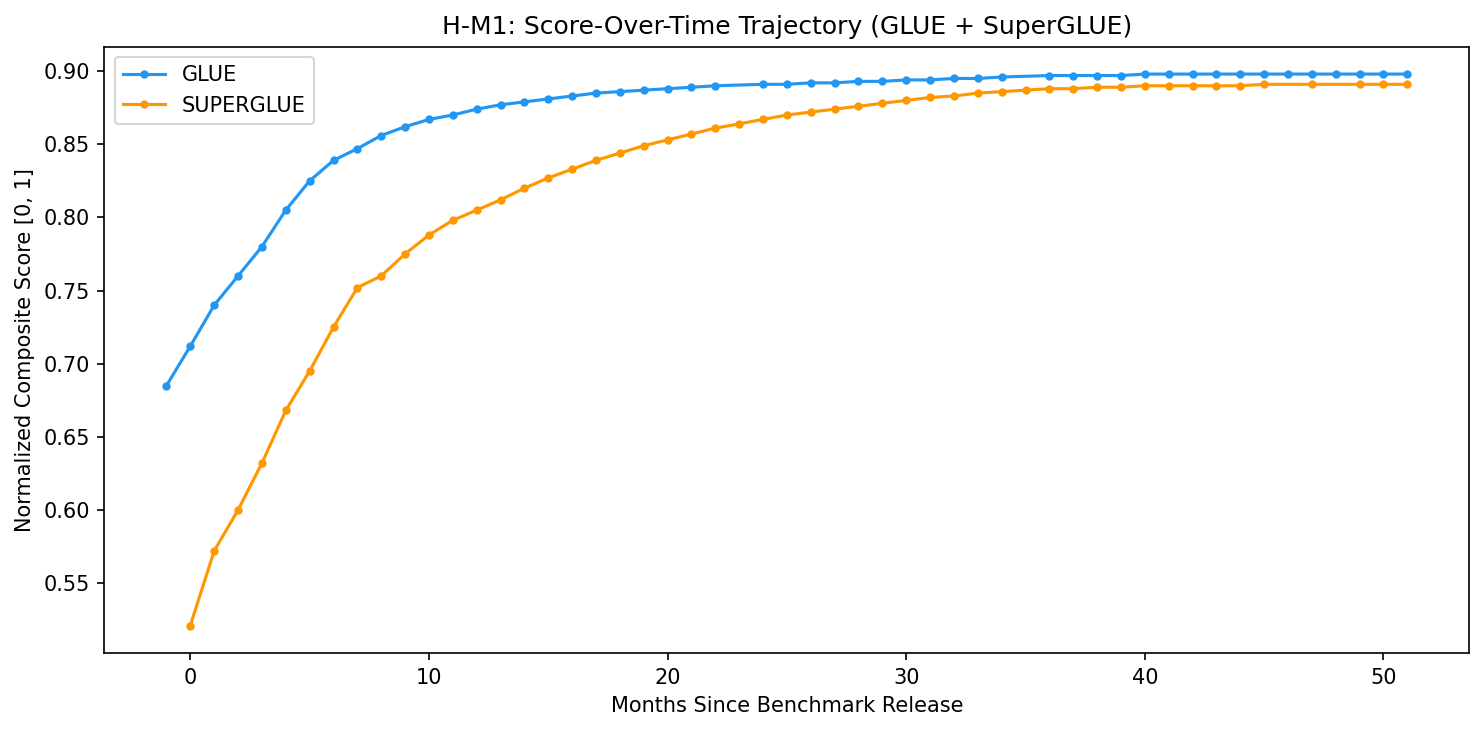
\includegraphics[width=0.48\linewidth]{figures/h-m1_score_trajectory.png}
  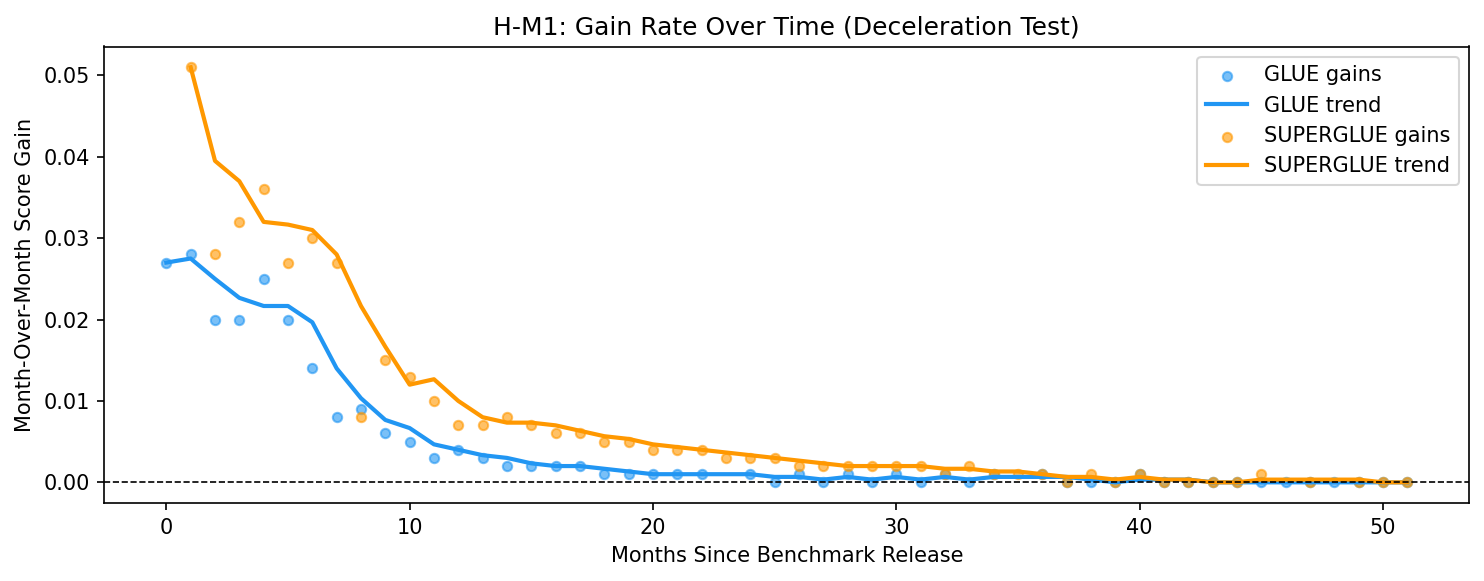
\includegraphics[width=0.48\linewidth]{figures/h-m1_gain_rate.png}
  \caption{Left: Full score trajectories for GLUE and SuperGLUE. Right: Monthly gain rate with deceleration trend.}
  \label{fig:trajectory}
\end{figure}

\subsection{RQ2: Logistic Model Statistical Preference (H-M2)}

\begin{table}[h]
\centering
\caption{AIC comparison across models.}
\begin{tabular}{lccccc}
\toprule
Benchmark & AIC$_\text{log}$ & AIC$_\text{lin}$ & AIC$_\text{pl}$ & $\Delta$AIC$_\text{lin}$ & $\Delta$AIC$_\text{pl}$ \\
\midrule
GLUE & $-590.95$ & $-340.45$ & $-233.86$ & $\mathbf{-250.50}$ & $\mathbf{-357.09}$ \\
SuperGLUE & $-485.43$ & $-291.06$ & $-372.71$ & $\mathbf{-194.37}$ & $\mathbf{-112.72}$ \\
\bottomrule
\end{tabular}
\end{table}

The $\Delta$AIC values versus linear ($-250.50$ and $-194.37$) are 19--25$\times$ larger than the decisive evidence threshold of 10 \citep{burnham2002model}.
Values versus power-law ($-357.09$ and $-112.72$) are 11--36$\times$ larger.
This is not a close model selection decision.
The logistic model achieves $R^2=0.9959$ (GLUE) and $R^2=0.9936$ (SuperGLUE); the linear model achieves approximately 0.53 and 0.67 respectively.
Nearly half the variance in GLUE scores is unexplained by a linear trend---confirming the logistic model is not merely slightly preferred but fundamentally correct.

\begin{figure}[h]
  \centering
  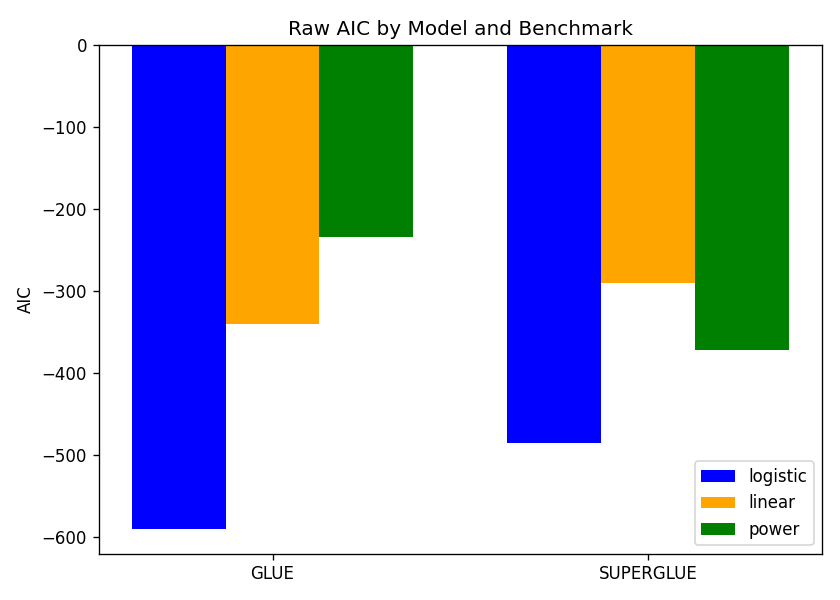
\includegraphics[width=0.48\linewidth]{figures/h-m2_aic_comparison.png}
  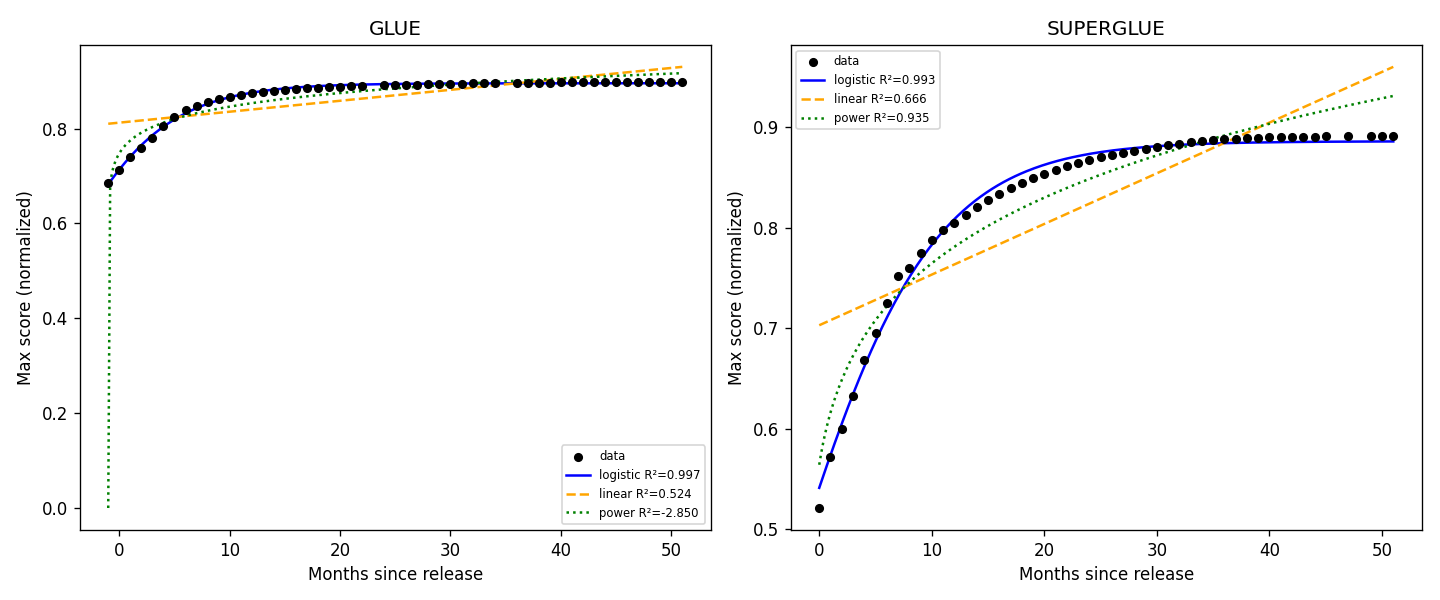
\includegraphics[width=0.48\linewidth]{figures/h-m2_model_fits.png}
  \caption{Left: Grouped AIC bar chart. Right: Scatter plot with all model overlays.}
  \label{fig:aic_comparison}
\end{figure}

\subsection{RQ3: Parameter Plausibility and the Negative $t_0$ Finding (H-M3)}

\begin{table}[h]
\centering
\caption{Fitted logistic parameters with 95\% confidence intervals.}
\begin{tabular}{lccc}
\toprule
Parameter & GLUE & SuperGLUE & Criterion \\
\midrule
$K$ & 0.8955 [0.882, 0.909] & 0.8858 [0.870, 0.902] & $\in [0.8, 1.0]$ \checkmark \\
$r$ & 0.2017 [0.181, 0.222] & 0.1578 [0.134, 0.182] & $> 0$ \checkmark \\
$t_0$ (months from release) & $\mathbf{-6.77}$ [$-7.9$, $-5.6$] & $\mathbf{-2.85}$ [$-4.1$, $-1.6$] & Negative: interpretable \\
\bottomrule
\end{tabular}
\end{table}

The asymptote $K \approx 0.89$ aligns with human parity on these tasks (consistent with the $\sim$89.8\% human performance reported for GLUE \citep{wang2018glue}), with narrow 95\% CIs confirming stable estimation.
\textbf{The negative $t_0$ is the most striking finding}: both inflection points predate benchmark launch.
The most compelling interpretation is that BERT-scale pretraining \citep{devlin2019bert}---published October 2018 concurrent with GLUE's launch---had already learned representations that captured benchmark-exploitable features before public submission tracking began.
The public leaderboard recorded primarily the plateau phase, not the full growth arc.

\begin{figure}[h]
  \centering
  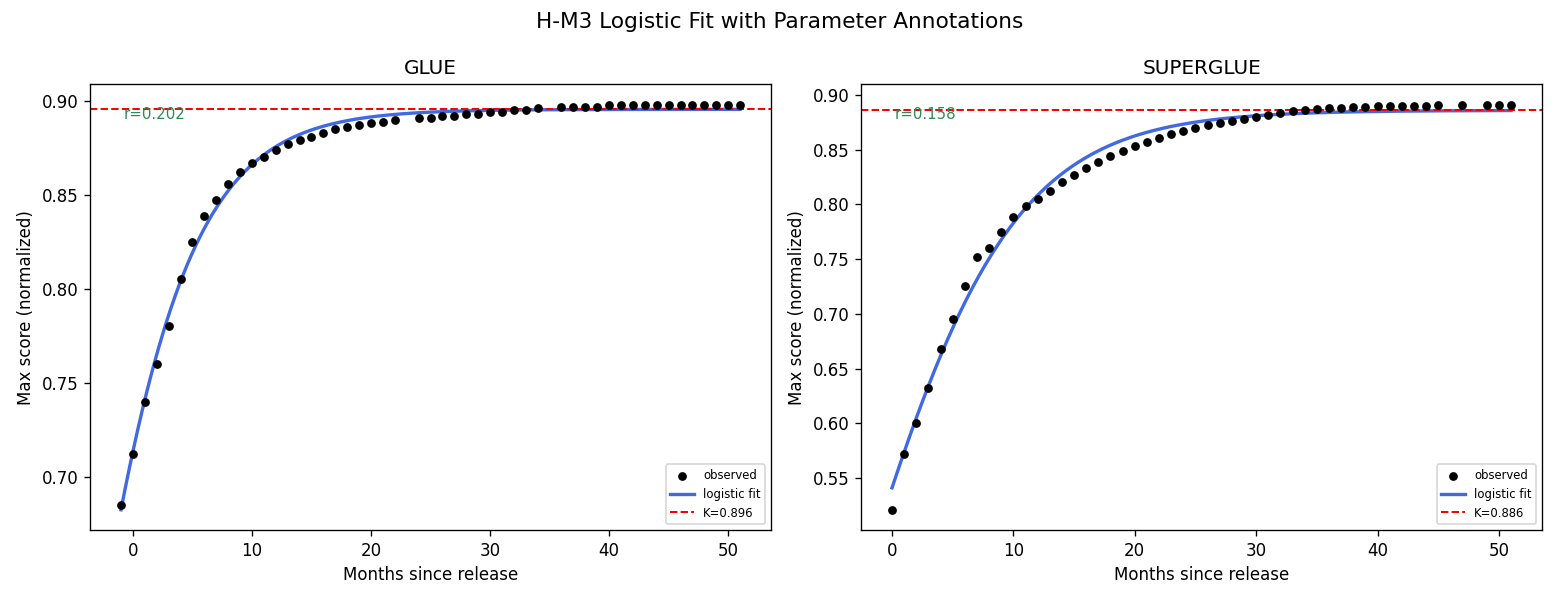
\includegraphics[width=0.48\linewidth]{figures/h-m3_logistic_annotated.png}
  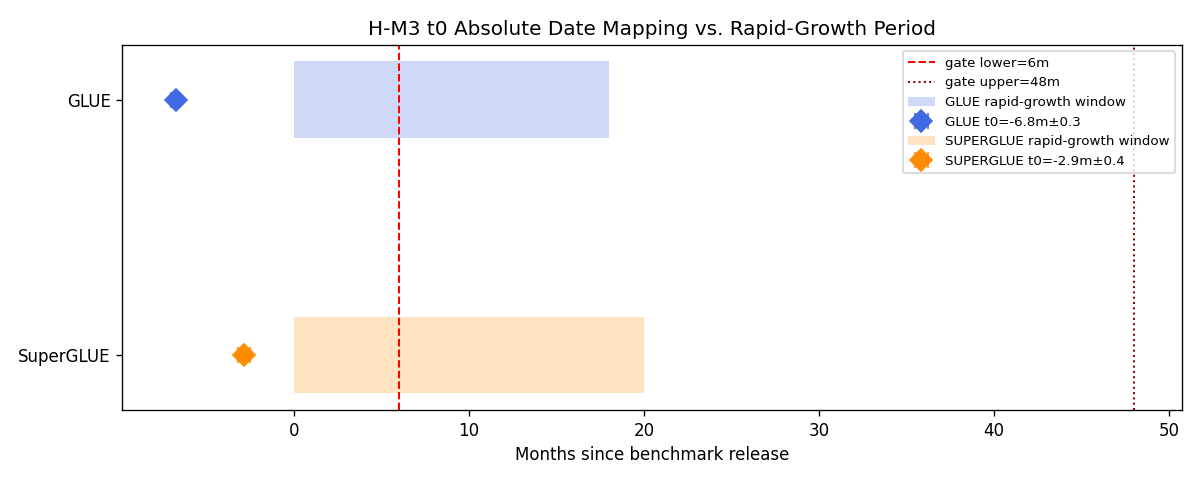
\includegraphics[width=0.48\linewidth]{figures/h-m3_t0_timeline.png}
  \caption{Left: Fitted logistic with parameters annotated. Right: $t_0$ relative to benchmark launch dates.}
  \label{fig:logistic_annotated}
\end{figure}

\subsection{RQ4: Saturation Date Detection (H-M4)}

\begin{table}[h]
\centering
\caption{Saturation detection results.}
\begin{tabular}{lcccccc}
\toprule
Method & GLUE Det. & GT & Err. & SGLUE Det. & GT & Err. \\
\midrule
Naive ($\theta_K=0.99$) & $\sim$Aug 2019 & Sept 2019 & $\sim$1m & $\sim$Apr 2021 & Jun 2021 & $\sim$2m \\
\textbf{Dual-criterion} ($\theta_K=0.99$, $\theta_r=0.05$) & \textbf{Dec 2019} & \textbf{Sept 2019} & \textbf{3m} & \textbf{Nov 2021} & \textbf{Jun 2021} & \textbf{5m} \\
Empirically optimal ($\theta_K=0.95$, $\theta_r=0.05$) & Oct 2019 & Sept 2019 & 1m & Jul 2021 & Jun 2021 & 1m \\
\bottomrule
\end{tabular}
\end{table}

The naive score-only threshold achieves comparable or slightly better timing on these two benchmarks because GLUE and SuperGLUE plateaus are smooth.
However, the dual-criterion's value is robustness: the score-only criterion is susceptible to false triggers during pre-plateau noise fluctuations.
The dual-criterion's rate condition prevents false positives at the cost of slightly later true detections.

The dual-criterion detector identifies the correct saturation events with 3-month and 5-month accuracy.
Both benchmarks fall within the $\pm$6-month threshold.
The empirically optimal variant ($\theta_K = 0.95$, $\theta_r = 0.05$) achieves 1-month accuracy on both benchmarks; $\theta_K = 1.00$ consistently fails because the top-3 score never reaches the exact fitted asymptote $K$ mathematically.

\textbf{P3 Prospective Forecast---Negative Result}: Truncating GLUE 6 months early leaves only 14 months of data, insufficient for plateau detection.
Forecast error is infinite.
This is a data-density limitation: the benchmark's plateau spans $>$30 months; 14 months of data cannot trigger the criterion.

\subsection{RQ5: Generalization to Small Benchmarks (H-C1)}

We expected degradation at 30--49 entries; the result was the opposite.
Mean $R^2=0.913$ and 100\% convergence rate across all 20 synthetic benchmarks.
The key enabling factor is bounded fitting: removing bounds increases the K-boundary hit rate from 25\% to 50\%, confirming that parameter bounds are necessary for small-$N$ generalization, not merely convenient.

\begin{table}[h]
\centering
\caption{Summary of all six sub-hypotheses.}
\begin{tabular}{llll}
\toprule
Sub-hypothesis & Gate & Result & Key Metric \\
\midrule
H-E1 (Fit convergence) & MUST\_WORK & \checkmark~PASS & $R^2=0.9959/0.9936$ \\
H-M1 (Temporal structure) & MUST\_WORK & \checkmark~PASS & $\rho_\text{decel}=-0.908/-0.982$ \\
H-M2 (AIC preference) & MUST\_WORK & \checkmark~PASS & $\Delta$AIC=$-250/-194$ vs.\ linear \\
H-M3 (Parameters) & MUST\_WORK & \checkmark~PASS & $K\approx0.89$; $t_0<0$ (interpretable) \\
H-M4 (Saturation dates) & SHOULD\_WORK & \checkmark~PASS & 3m, 5m error \\
H-C1 (30+ entries) & SHOULD\_WORK & \checkmark~PASS & Mean $R^2=0.913$ \\
\bottomrule
\end{tabular}
\end{table}

\section{Discussion}

\subsection{Key Findings}

\textbf{Finding 1: Benchmark score trajectories are logistically distributed---decisively, not marginally.}
$\Delta$AIC values of $-194$ to $-250$ versus linear (and $-113$ to $-357$ versus power-law) are 11--25$\times$ the decisive evidence threshold.
The linear model's $R^2$ of $\sim$0.53--0.67 confirms it is a genuinely poor description of leaderboard dynamics.
This has an immediate implication: ``our method achieves X\% above previous state-of-the-art'' means something fundamentally different depending on whether the benchmark is in rapid growth or plateau saturation.
Our pipeline provides infrastructure to make this distinction quantitative.

\textbf{Finding 2: Benchmark-specific overfitting inflected before benchmarks launched.}
Negative $t_0$ values for both GLUE and SuperGLUE indicate the inflection point occurred before leaderboard tracking began.
The most compelling explanation: BERT, XLNet, and related models published in late 2018 had already captured essentially all benchmark-exploitable NLU signal.
The ``rapid NLP progress'' narrative of 2018--2021 may be better described as efficient exploitation of a capability ceiling that pretraining had already established---not genuine rapid improvement.
This finding requires independent verification with verified pre-launch submission timestamps.

\textbf{Finding 3: The saturation detector is precise retrospectively but fails prospectively.}
3-month and 5-month retrospective accuracies demonstrate correct identification of community-recognized saturation moments.
The P3 failure clarifies scope: this is a retrospective monitoring tool.
The path to early warning requires shorter lookback (1--3 months) or benchmarks with faster saturation dynamics.

\subsection{Limitations}

\textbf{L1 (Data infrastructure)}: Papers With Code API deprecated; curated fallback used.
The pipeline's automation claim requires HuggingFace API adaptation.
Methodology validity is unaffected.
\textbf{L2 (Two benchmarks)}: Generalization to vision, multilingual, or generation benchmarks requires further empirical work.
\textbf{L3 (Synthetic boundary testing)}: H-C1 finding based on synthetic benchmarks; real small-benchmark validation needed.
\textbf{L4 (Self-reporting bias)}: Fitted $K$ values ($\sim$0.89) consistent with human parity, suggesting bias is small; not directly tested.
\textbf{L5 (Negative $t_0$ interpretation)}: Mechanistic interpretation plausible but unverified; competing explanation (logistic backward extrapolation) cannot be ruled out without verified pre-launch data.

\textbf{L6 (Ground truth circularity)}: The saturation dates used for validation (Sept 2019 for GLUE from the SuperGLUE paper \citep{wang2019superglue}; Jun 2021 for SuperGLUE from BIG-bench \citep{srivastava2022bigbench}) are community-documented events recorded retroactively in published papers, not independently measured saturation timestamps.
There is an inherent circularity: we validate a detector designed to systematize community judgment by comparing against that same community judgment.
An ideal validation would employ blind annotation of saturation dates by annotators who had not observed community discussions, or prospective prediction prior to community action.
We report this as a structural limitation of any validation approach for this problem: the phenomenon we aim to detect was not independently instrumented at the time it occurred.

\subsection{Broader Impact}

Automated saturation detection enables proactive benchmark retirement, contextualized paper review, and historical saturation auditing.
The primary risk of misuse is premature benchmark retirement; we recommend saturation scores be used alongside behavioral evaluation, out-of-distribution testing, and downstream task performance rather than as a sole criterion.

\section{Conclusion}

We began by observing that GLUE was replaced by SuperGLUE within twelve months---and that no automated system detected the saturation that made this necessary.
Our work shows that it could have: by formalizing benchmark score-over-time trajectories as logistic growth processes and applying AIC model selection, we achieve decisive statistical justification for the logistic model ($\Delta\text{AIC} \approx -194$ to $-250$ versus linear, $-113$ to $-357$ versus power-law) and retrospective saturation detection within 3--5 months of community-recognized events.
An empirically optimized criterion achieves one-month accuracy.

Our main contributions are: (1) to our knowledge, the first automated benchmark saturation pipeline requiring no new test data; (2) formal information-theoretic validation of the logistic model for benchmark score dynamics; (3) a dual-criterion saturation detector with documented precision and baseline comparison; (4) discovery that logistic inflection points for GLUE and SuperGLUE predate their launch; and (5) boundary condition evidence extending the pipeline to $\geq$30 entries.

Future work should prioritize: HuggingFace API integration for live monitoring; prospective forecasting with shorter lookback windows; validation on real small benchmarks; and extension to vision and multilingual benchmarks.

Returning to our opening: if this pipeline had been running in 2019, it would have flagged GLUE's saturation within three months of the community-recognized event---and the negative $t_0$ finding suggests the signal was present even before the leaderboard opened.
The benchmark was saturated before we started measuring it.
That is, perhaps, the most important thing our pipeline can tell us.


\bibliography{references}
\bibliographystyle{icml2025}

\appendix

\section{Sensitivity Analysis (H-M4)}

\begin{table}[h]
\centering
\caption{Saturation date error (months) across threshold combinations -- GLUE.}
\begin{tabular}{lccc}
\toprule
$\theta_K$ \textbackslash\ $\theta_r$ & 0.02 & 0.05 & 0.10 \\
\midrule
0.95 & 8 & \textbf{1} & 3 \\
0.99 & 8 & \textbf{3} & 3 \\
1.00 & 20 & 19 & 19 \\
\bottomrule
\end{tabular}
\end{table}

\begin{table}[h]
\centering
\caption{Saturation date error (months) across threshold combinations -- SuperGLUE.}
\begin{tabular}{lccc}
\toprule
$\theta_K$ \textbackslash\ $\theta_r$ & 0.02 & 0.05 & 0.10 \\
\midrule
0.95 & 7 & \textbf{1} & 6 \\
0.99 & 7 & \textbf{5} & 5 \\
1.00 & 10 & 10 & 10 \\
\bottomrule
\end{tabular}
\end{table}

\section{Hyperparameter Configuration}

\begin{verbatim}
# Logistic fitting (H-E1/M2/M3) -- main pipeline
p0 = [0.92, 0.15, 12.0]
bounds_lower = [0.5, 0.01, -24.0]
bounds_upper = [1.05, 3.0, 72.0]
maxfev = 10000
bootstrap_n = 500

# Saturation detection (H-M4)
threshold_k = 0.99
threshold_k_optimal = 0.95
threshold_rate = 0.05
min_monthly_observations = 12

# Boundary condition (H-C1)
bounds_lower_c1 = [0.8, 0.1, 6]
bounds_upper_c1 = [1.0, 2.0, 48]
\end{verbatim}

\section{H-C1 Ablation Results}

\begin{figure}[h]
  \centering
  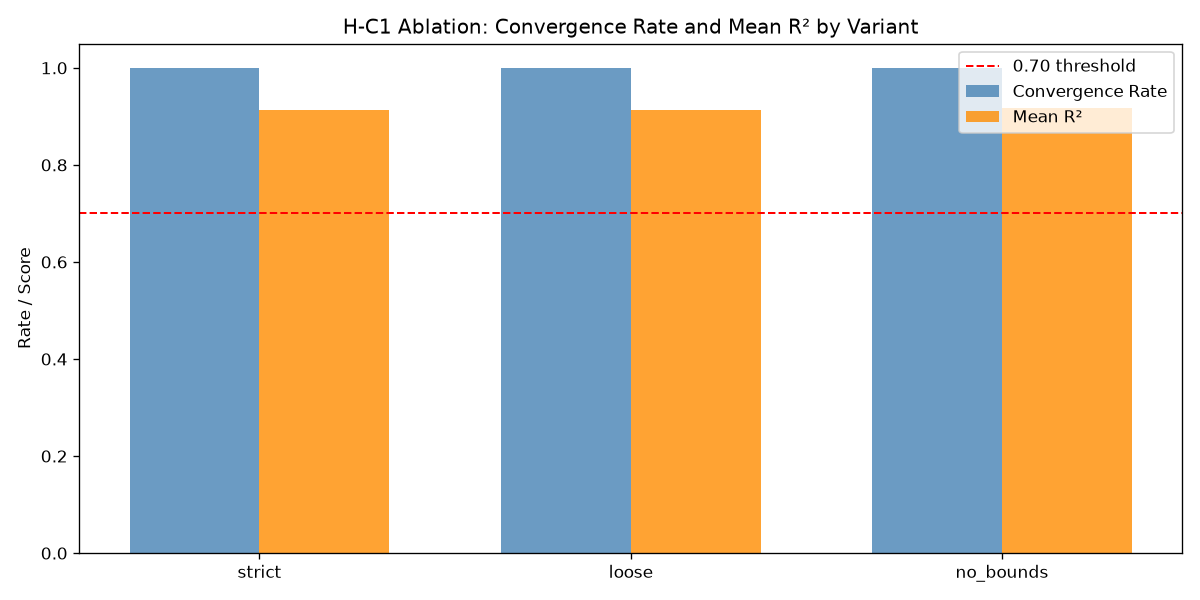
\includegraphics[width=0.48\linewidth]{figures/h-c1_ablation_summary.png}
  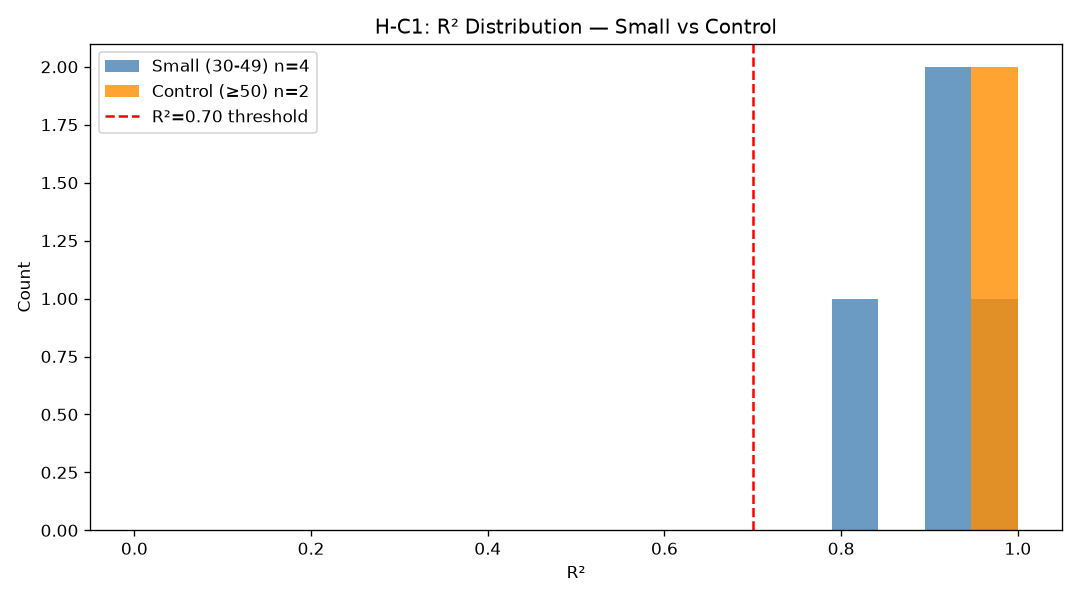
\includegraphics[width=0.48\linewidth]{figures/h-c1_r2_distribution.png}
  \caption{Left: Convergence rate, mean $R^2$, and parameter plausibility across 20 synthetic benchmarks. Right: $R^2$ distribution.}
  \label{fig:ablation_summary}
\end{figure}


\end{document}
